\documentclass[12pt,a4paper]{report}

% ---------- Packages ----------
\usepackage[T1]{fontenc}
\usepackage[utf8]{inputenc}
\usepackage{mathptmx}
\usepackage[a4paper,left=2.5cm,right=2.5cm,top=2.5cm,bottom=2.5cm]{geometry}
\usepackage{graphicx}
\usepackage[table]{xcolor}
\usepackage{array,tabularx,longtable,booktabs}
\usepackage{enumitem}
\usepackage{caption}
\usepackage{fancyhdr}
\usepackage{titlesec}
\usepackage{tikz}
\usetikzlibrary{arrows.meta,positioning,calc,fit,backgrounds}
\usepackage[hidelinks]{hyperref}
\usepackage{setspace}
\usepackage{float}
\usepackage[most]{tcolorbox}
\newtcolorbox{example}[1][]{colback=boxfill,colframe=boxline,boxrule=0.6pt,arc=2pt,left=8pt,right=8pt,top=6pt,bottom=6pt,fonttitle=\bfseries\small,coltitle=white,colbacktitle=tablehead,title={#1}}

% ---------- Colours ----------
\definecolor{headteal}{HTML}{1B4A4A}
\definecolor{tablehead}{HTML}{153F3F}
\definecolor{rowtint}{HTML}{F1F6F5}
\definecolor{boxfill}{HTML}{E6F2EF}
\definecolor{boxline}{HTML}{3D8C80}
\definecolor{sand}{HTML}{F6E7CF}
\definecolor{sandline}{HTML}{D9A766}
\definecolor{gantt}{HTML}{2E8B7E}

% ---------- Layout ----------
\setstretch{1.15}
\setlength{\parindent}{0pt}
\setlength{\parskip}{6pt}
\pagestyle{fancy}
\fancyhf{}
\fancyhead[L]{\small AI Legal Intelligence \& Assistance Platform for Pakistan}
\fancyfoot[C]{\thepage}
\renewcommand{\headrulewidth}{0pt}
\fancypagestyle{plain}{\fancyhf{}\fancyhead[L]{\small AI Legal Intelligence \& Assistance Platform for Pakistan}\fancyfoot[C]{\thepage}\renewcommand{\headrulewidth}{0pt}}

\titleformat{\chapter}[hang]{\normalfont\LARGE\bfseries\color{headteal}}{\thechapter}{0.6em}{}
\titlespacing*{\chapter}{0pt}{0pt}{12pt}
\titleformat{\section}{\normalfont\Large\bfseries\color{headteal}}{\thesection}{0.5em}{}
\titleformat{\subsection}{\normalfont\large\bfseries}{\thesubsection}{0.5em}{}

\renewcommand{\contentsname}{\color{headteal}Table of Contents}
\renewcommand{\listfigurename}{\color{headteal}List of Figures}
\renewcommand{\listtablename}{\color{headteal}List of Tables}
\setcounter{tocdepth}{2}
\renewcommand{\thefigure}{\arabic{figure}}
\renewcommand{\thetable}{\arabic{table}}
\captionsetup{font={small,it},labelfont={small,it},labelsep=colon}
\captionsetup[table]{position=top,skip=4pt}

\setlist[itemize]{label=\textbullet,leftmargin=1.5em,itemsep=2pt,topsep=2pt}
\setlist[enumerate]{leftmargin=1.8em,itemsep=2pt,topsep=2pt}

% Table helpers
\newcolumntype{L}[1]{>{\raggedright\arraybackslash}p{#1}}
\newcommand{\thd}[1]{\textcolor{white}{\textbf{#1}}}
\newcommand{\headrow}{\rowcolor{tablehead}}
\renewcommand{\arraystretch}{1.3}

% TikZ styles
\tikzset{
  wstep/.style={draw=boxline,fill=boxfill,rounded corners=2pt,align=center,font=\footnotesize,minimum height=0.9cm,text width=2.3cm,inner sep=3pt},
  dark/.style={wstep,fill=tablehead,text=white},
  flow/.style={-{Stealth[length=2mm]},thick,color=headteal},
}

\begin{document}

% ================= TITLE PAGE =================
\begin{titlepage}
\thispagestyle{plain}
\centering
\vspace*{1.5cm}
{\fontsize{24}{30}\selectfont\bfseries AI Powered Legal Advisor and Analyzer\par}
\vspace{0.8cm}
\includegraphics[width=4.2cm]{figures/cust_logo.png}\par
\vspace{0.8cm}
{\Large\bfseries Final Year Project Proposal\par}
\vspace{0.1cm}
{\large Design Project (Part-I)\par}
\vspace{0.6cm}
{\large\bfseries Team Members\par}
\vspace{0.1cm}
{\large Muhammad Nabeel (BCS233115)\par Ashir Qureshi (BCS233084)\par Muhammad Sharjeel (BCS233113)\par}
\vspace{0.5cm}
{\large\bfseries Supervised By\par}
\vspace{0.1cm}
{\large Ms. Khadija Iftikhar\par}
\vspace{0.5cm}
{\large Fall 2026\par}
\vspace{0.2cm}
{\large Bachelor of Science in Computer Science\par}
{\large\bfseries Department of Computer Science\par}
{\large Capital University of Science \& Technology, Islamabad\par}
\vfill
\end{titlepage}
\setcounter{page}{2}

\tableofcontents
\clearpage
\listoffigures
\vspace{1em}
\listoftables
\clearpage

% ================= CHAPTER 1 =================
\chapter*{Introduction}
\addcontentsline{toc}{chapter}{Chapter 1 --- Introduction}
\setcounter{chapter}{1}
\setcounter{section}{0}

\section{Project Introduction}

\subsection{Project Goal}
Our goal is simple: build an AI platform that lets an ordinary Pakistani citizen understand a property or family legal problem in plain words, based on verified Pakistani legal sources, and then reach a lawyer who can actually help. Everything on the platform is organized around the user's case, not around isolated questions.

\subsection{Problem Statement}
For most people, the law feels out of reach. The relevant acts, rules and court procedures are scattered across many documents, and they are written for lawyers rather than for the people they affect. Someone facing a tenancy, inheritance, divorce or custody issue usually has three questions and no one to ask: Which law applies to me? What papers should I collect? Which lawyer should I go to?

AI chatbots seem like an easy answer, and they do reply quickly. The trouble is that a general chatbot does not necessarily draw on verified Pakistani law, and it can state things confidently that turn out to be wrong or impossible to check. In a legal matter, that kind of mistake can cost someone their home or their rights.

\begin{example}[Example: Ali's situation]
Ali rents a house in Lahore. One evening his landlord calls and tells him to leave within seven days. Ali has a written rent agreement, but he has never read the rent law, he does not know whether a phone call counts as notice, and he has no idea which lawyer to trust. This is exactly the kind of person we are building for, and we use his case as a running example in this proposal.
\end{example}

\subsection{Objectives}
We have set ourselves six concrete objectives:
\begin{enumerate}
  \item Build a verified knowledge base of Pakistani legal sources covering property and family disputes.
  \item Develop a RAG-based assistant that answers only from retrieved legal text and always shows where each answer came from.
  \item Ask only the follow-up questions that are really needed to understand a case before giving any guidance.
  \item Read uploaded documents (PDFs and scanned images) and turn them into an evidence checklist for that specific case.
  \item Offer a directory of verified lawyers with useful search filters, and track each case until it is resolved.
  \item Compare our system with a standard LLM on defined quality measures, and test how easy it is to use.
\end{enumerate}

\subsection{Proposed Solution}
The platform brings three things together in one place:
\begin{itemize}
  \item \textbf{A RAG-based legal assistant.} Instead of answering from the model's memory, it first looks up the relevant sections in our verified legal knowledge base and builds the answer from them. The sources are shown next to the answer, so anyone can check it.
  \item \textbf{A verified lawyer directory.} An administrator checks every lawyer profile before it goes live. Users can then narrow down the list by specialization, city and other filters.
  \item \textbf{Case tracking.} A case stays open from the first question until it is resolved, so the user can always see where things stand and what comes next.
\end{itemize}

\subsection{Users}
\begin{table}[H]
\centering
\caption{Users of the platform and their roles}
\label{tab:users}
\begin{tabular}{|L{3.6cm}|L{10.4cm}|}
\hline
\headrow \thd{User} & \thd{Role on the platform} \\ \hline
\textbf{Citizen} & Main user. Creates cases, answers follow-up questions, uploads documents, reads guidance, searches lawyers and follows case progress. \\ \hline
\rowcolor{rowtint}\textbf{Lawyer} & Maintains a professional profile and accesses cases that a citizen has chosen to share with them. \\ \hline
\textbf{Administrator} & Manages users, lawyers, cases and legal content, and verifies lawyers before they appear in the directory. \\ \hline
\end{tabular}
\end{table}

\subsection{System Workflow}
Figure~\ref{fig:workflow} shows the journey of a case through the platform. It has nine steps.

\begin{figure}[H]
\centering
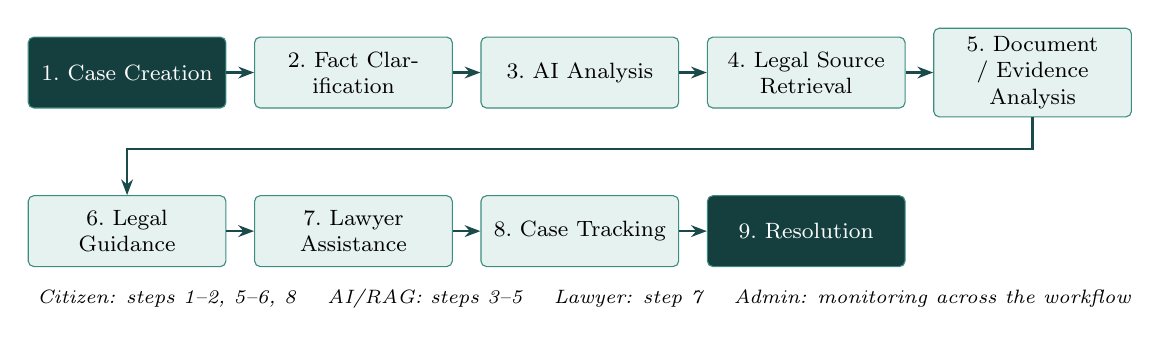
\begin{tikzpicture}[node distance=0.35cm]
  \node[dark] (s1) {1.\ Case Creation};
  \node[wstep,right=of s1] (s2) {2.\ Fact Clarification};
  \node[wstep,right=of s2] (s3) {3.\ AI Analysis};
  \node[wstep,right=of s3] (s4) {4.\ Legal Source Retrieval};
  \node[wstep,right=of s4] (s5) {5.\ Document / Evidence Analysis};
  \node[wstep,below=1.1cm of s1] (s6) {6.\ Legal Guidance};
  \node[wstep,right=of s6] (s7) {7.\ Lawyer Assistance};
  \node[wstep,right=of s7] (s8) {8.\ Case Tracking};
  \node[dark,right=of s8] (s9) {9.\ Resolution};
  \foreach \a/\b in {s1/s2,s2/s3,s3/s4,s4/s5,s6/s7,s7/s8,s8/s9} \draw[flow] (\a) -- (\b);
  \draw[flow] (s5.south) -- ++(0,-0.4) -| (s6.north);
  \node[below=0.15cm of s6.south west,anchor=north west,font=\scriptsize\itshape] {Citizen: steps 1--2, 5--6, 8 \quad AI/RAG: steps 3--5 \quad Lawyer: step 7 \quad Admin: monitoring across the workflow};
\end{tikzpicture}
\caption{Main workflow of the proposed platform}
\label{fig:workflow}
\end{figure}

\begin{enumerate}
  \item \textbf{Case creation.} The user explains the problem in their own words.
  \item \textbf{Fact clarification.} If something important is missing, the system asks a short follow-up question, for example whether there is a written tenancy agreement or whether the marriage was registered.
  \item \textbf{AI analysis.} The system looks at the facts and works out which legal topics are involved.
  \item \textbf{Legal source retrieval.} The RAG component pulls the most relevant legal sources out of the knowledge base (Figure~\ref{fig:rag}).
  \item \textbf{Document / evidence analysis.} If the user uploads papers such as an agreement or a notice, the system reads them. PyMuPDF handles normal PDFs, OCR handles scans and photos, and the important clauses are picked out.
  \item \textbf{Legal guidance.} The user gets a plain-language explanation with citations, along with a checklist of documents and evidence to keep ready.
  \item \textbf{Lawyer assistance.} If needed, the user finds a suitable lawyer (Figure~\ref{fig:lawyer}) and chooses to share the case with them.
  \item \textbf{Case tracking.} The user keeps an eye on the case status from the platform.
  \item \textbf{Resolution.} Once the matter is settled, the case is closed.
\end{enumerate}
In short, the citizen is involved in steps 1, 2, 5, 6 and 8, the AI/RAG part does the work in steps 3 to 5, the lawyer comes in at step 7, and the administrator keeps an eye on the whole process.

\begin{example}[Example: Ali's case through the workflow]
\textbf{Step 1:} Ali types, ``My landlord says I must leave in 7 days.''\\
\textbf{Step 2:} The system asks, ``Do you have a written agreement? Did you receive a written notice?'' Ali says he has an agreement but only got a phone call.\\
\textbf{Steps 3--5:} The system identifies a tenancy and eviction issue, retrieves the matching rent law sections, and reads the agreement Ali uploads.\\
\textbf{Step 6:} Ali gets a short explanation with citations and a checklist: agreement, rent receipts, a record of the call.\\
\textbf{Steps 7--9:} He filters lawyers by \emph{Property} and \emph{Lahore}, shares his case with one of them, and follows it until it is closed.\\[2pt]
{\small\itshape This example is illustrative and does not describe actual legal advice.}
\end{example}

\subsection{Scope}
We are deliberately starting small. The first version covers only the two areas in Figure~\ref{fig:scope}, and nothing else. A narrow, carefully checked knowledge base is far more useful than a broad one that nobody can trust.

\begin{figure}[H]
\centering
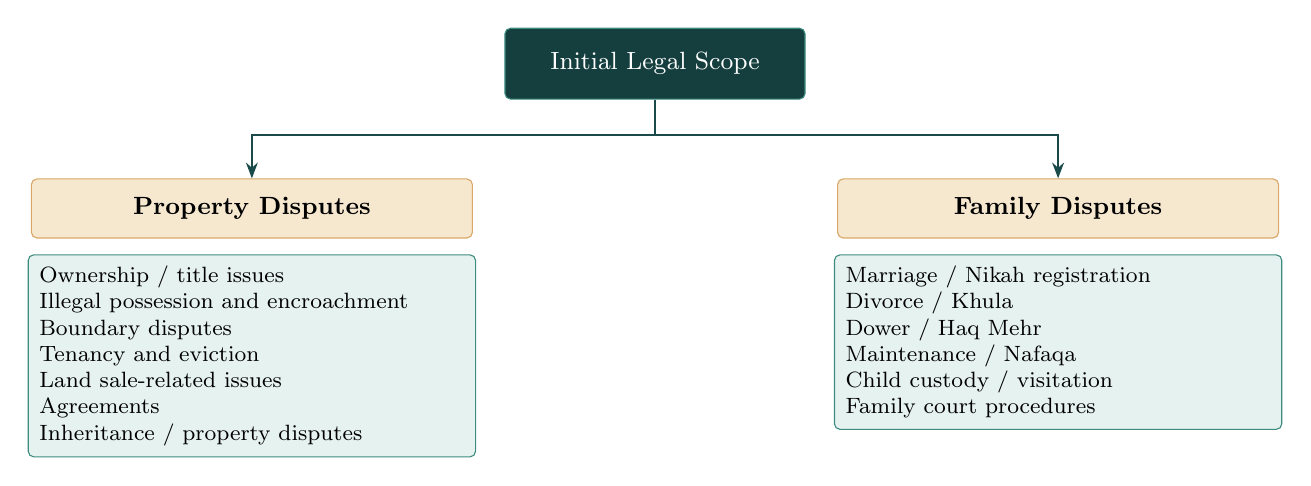
\begin{tikzpicture}[
  area/.style={draw=sandline,fill=sand,rounded corners=2pt,font=\small\bfseries,minimum width=5.6cm,minimum height=0.75cm},
  list/.style={draw=boxline,fill=boxfill,rounded corners=2pt,font=\footnotesize,text width=5.4cm,align=left,inner sep=4pt}]
  \node[dark,text width=3.6cm,font=\small] (root) {Initial Legal Scope};
  \node[area,below left=1.0cm and 0.4cm of root] (p) {Property Disputes};
  \node[area,below right=1.0cm and 0.4cm of root] (f) {Family Disputes};
  \node[list,below=0.2cm of p] {Ownership / title issues\\Illegal possession and encroachment\\Boundary disputes\\Tenancy and eviction\\Land sale-related issues\\Agreements\\Inheritance / property disputes};
  \node[list,below=0.2cm of f,anchor=north] (fl) {Marriage / Nikah registration\\Divorce / Khula\\Dower / Haq Mehr\\Maintenance / Nafaqa\\Child custody / visitation\\Family court procedures};
  \draw[flow] (root.south) -- ++(0,-0.45) -| (p.north);
  \draw[flow] (root.south) -- ++(0,-0.45) -| (f.north);
\end{tikzpicture}
\caption{Initial legal scope --- Property Disputes and Family Disputes}
\label{fig:scope}
\end{figure}

\begin{table}[H]
\centering
\caption{Initial legal scope and topics covered}
\label{tab:scope}
\begin{tabular}{|L{3.6cm}|L{10.4cm}|}
\hline
\headrow \thd{Area} & \thd{Topics covered} \\ \hline
\textbf{Property Disputes} & Ownership / title issues; illegal possession and encroachment; boundary disputes; tenancy and eviction; land sale-related issues; agreements; inheritance / property disputes. \\ \hline
\rowcolor{rowtint}\textbf{Family Disputes} & Marriage / Nikah registration; divorce / Khula; dower / Haq Mehr; maintenance / Nafaqa; child custody / visitation; family court procedures. \\ \hline
\end{tabular}
\end{table}

\subsection{Expected Benefits}
\begin{itemize}
  \item \textbf{Citizens} get legal information they can actually understand, with sources they can trace, a clear idea of what evidence to prepare, and an easier way to find the right lawyer.
  \item \textbf{Lawyers} receive cases that arrive organized and well documented, which saves time on both sides.
  \item \textbf{Administrators} get one place to manage users, lawyers, cases and legal content.
\end{itemize}
We want to be clear about one thing: the platform helps people understand their situation, but it \textbf{does not replace a qualified lawyer}. Anything that needs professional judgment should still go to one.

\begin{figure}[H]
\centering
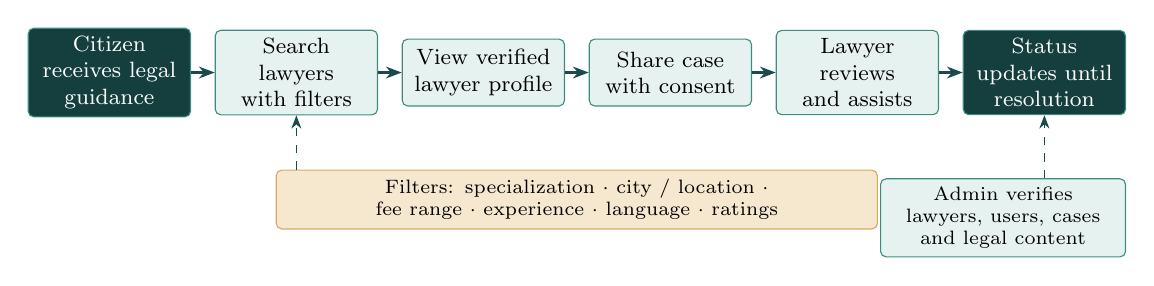
\begin{tikzpicture}[node distance=0.3cm, s/.style={wstep,text width=1.85cm,minimum height=0.85cm}, d/.style={dark,text width=1.85cm,minimum height=0.85cm}]
  \node[d] (a) {Citizen receives legal guidance};
  \node[s,right=of a] (b) {Search lawyers with filters};
  \node[s,right=of b] (c) {View verified lawyer profile};
  \node[s,right=of c] (d) {Share case with consent};
  \node[s,right=of d] (e) {Lawyer reviews and assists};
  \node[d,right=of e] (g) {Status updates until resolution};
  \foreach \x/\y in {a/b,b/c,c/d,d/e,e/g} \draw[flow] (\x) -- (\y);
  \node[draw=sandline,fill=sand,rounded corners=2pt,font=\scriptsize,below=0.8cm of c.south west,anchor=north west,xshift=-1.6cm,text width=7.4cm,align=center] (filt) {Filters: specialization $\cdot$ city / location $\cdot$ fee range $\cdot$ experience $\cdot$ language $\cdot$ ratings};
  \node[wstep,font=\scriptsize,text width=2.9cm,below=0.8cm of g.south east,anchor=north east] (adm) {Admin verifies lawyers, users, cases and legal content};
  \draw[-{Stealth},dashed,color=headteal] (filt.north -| b.south) -- (b.south);
  \draw[-{Stealth},dashed,color=headteal] (adm.north -| g.south) -- (g.south);
\end{tikzpicture}
\caption{Lawyer discovery and case progress}
\label{fig:lawyer}
\end{figure}

Figure~\ref{fig:lawyer} shows how a citizen moves from guidance to a lawyer. They search using filters such as specialization, city, fee range, experience, language and ratings, open a verified profile, share the case only if they agree to, and then receive updates until the matter is resolved. Behind the scenes, the administrator keeps verifying lawyers, users, cases and legal content.

\section{Existing Examples / Solutions}
Two Pakistani platforms come closest to what we are building: MyCounsel and QanoonAI. What follows is based on their public descriptions in the Stanford CodeX TechIndex (last reviewed July 2026). We have not used these products ourselves, so where a feature is not mentioned we mark it as ``not stated'' instead of assuming it does not exist.

\subsection*{Competitor 1: MyCounsel}
\begin{table}[H]
\centering
\caption{Profile of MyCounsel}
\label{tab:mycounsel}
\begin{tabular}{|L{3.4cm}|L{10.6cm}|}
\hline
\headrow \thd{Aspect} & \thd{Description} \\ \hline
\textbf{Background} & A Pakistani legal platform combining a lawyer marketplace with AI legal research tools. It serves both consumers and law firms. \\ \hline
\rowcolor{rowtint}\textbf{Purpose} & To make it easier to find lawyers and to support professional legal work online. \\ \hline
\textbf{Main functionality} & Clients can search verified lawyers, book paid consultations, and manage engagements, messages and documents online. Firms and in-house teams can use shared workflows, centralized billing and AI research over Pakistani case law and law journals. \\ \hline
\rowcolor{rowtint}\textbf{How it works} & The user searches the lawyer marketplace, books a consultation and continues the engagement through the platform, while professional users use the AI research tools. \\ \hline
\textbf{Strengths} & Verified lawyer search, online booking and engagement management, and AI research over Pakistani legal material. \\ \hline
\rowcolor{rowtint}\textbf{Limitations} & The public description does not mention fact-clarifying follow-up questions for a citizen's case, evidence checklists, OCR, or a retrieval-grounded explanation of the user's situation with citations. \\ \hline
\end{tabular}
\end{table}

\subsection*{Competitor 2: QanoonAI}
\begin{table}[H]
\centering
\caption{Profile of QanoonAI}
\label{tab:qanoonai}
\begin{tabular}{|L{3.4cm}|L{10.6cm}|}
\hline
\headrow \thd{Aspect} & \thd{Description} \\ \hline
\textbf{Background} & An AI legal intelligence platform focused on Pakistani law, aimed at judges, lawyers and citizens. Citizens have free access and professional users have paid plans. \\ \hline
\rowcolor{rowtint}\textbf{Purpose} & To give faster access to Pakistani judgments and legal research support. \\ \hline
\textbf{Main functionality} & A database of Pakistani judgments with tools for neutral case briefs, petition drafting, citation verification, court-fee calculation and Urdu-language legal guidance. \\ \hline
\rowcolor{rowtint}\textbf{How it works} & Users query the judgment database and use the drafting, verification and calculation tools. \\ \hline
\textbf{Strengths} & Pakistani legal focus, judgment database, citation verification and Urdu-language support. \\ \hline
\rowcolor{rowtint}\textbf{Limitations} & The public description is centered on judgments and professional tools. It does not mention a lawyer directory, case tracking, evidence checklists or OCR. \\ \hline
\end{tabular}
\end{table}

\subsection*{Comparison}
\begin{table}[H]
\centering
\caption[Comparison of existing solutions and the proposed system]{Comparison of existing solutions and the proposed system. ``Not stated'' means the public description does not mention the feature.}
\label{tab:comparison}
\begin{tabular}{|L{3.2cm}|L{3.3cm}|L{3.3cm}|L{3.8cm}|}
\hline
\headrow \thd{Feature} & \thd{MyCounsel} & \thd{QanoonAI} & \thd{Proposed System (planned)} \\ \hline
\textbf{Legal information} & AI research on case law and journals & Judgments, case briefs & Property and family law information \\ \hline
\rowcolor{rowtint}\textbf{Pakistani legal focus} & Yes & Yes & Yes \\ \hline
\textbf{Case-based analysis} & Not stated & Case briefs & Analysis of the user's case facts \\ \hline
\rowcolor{rowtint}\textbf{RAG / grounded responses} & Not stated & Not stated & Yes \\ \hline
\textbf{Source citations} & Not stated & Citation verification & Yes \\ \hline
\rowcolor{rowtint}\textbf{Follow-up questions} & Not stated & Not stated & Yes \\ \hline
\textbf{Document processing} & Online document sharing & Petition drafting & PDF text and clause extraction \\ \hline
\rowcolor{rowtint}\textbf{OCR} & Not stated & Not stated & Yes \\ \hline
\textbf{Evidence checklist} & Not stated & Not stated & Yes \\ \hline
\rowcolor{rowtint}\textbf{Lawyer directory} & Yes (verified lawyers) & Not stated & Yes (verified lawyers) \\ \hline
\textbf{Lawyer filtering} & Search & Not stated & Specialization, city, fee, experience, language, rating \\ \hline
\rowcolor{rowtint}\textbf{Case tracking} & Engagement management & Not stated & Yes \\ \hline
\end{tabular}
\end{table}

\textbf{Where the gap is.} Both platforms are useful, but they are built mainly for professionals: one focuses on finding lawyers and legal research, the other on judgments and drafting. What is missing is a simple path for an ordinary citizen. Our system fills that gap with one case-centered workflow: it clarifies the facts, finds verified sources, explains them in plain language with citations, tells the user what evidence to prepare, connects them to a suitable lawyer, and tracks the case, all within property and family disputes.

\section{Business Scope}
This section looks at who the platform is for and where it could go after the FYP. The commercial ideas below are \emph{possibilities}, not promises; none of them is confirmed revenue.

\begin{table}[H]
\centering
\caption{Business scope of the platform}
\label{tab:business}
\begin{tabular}{|L{3.6cm}|L{10.4cm}|}
\hline
\headrow \thd{Item} & \thd{Description} \\ \hline
\textbf{Target market} & Pakistani citizens, especially people facing property or family disputes, people who want understandable legal information, and people looking for relevant lawyers. \\ \hline
\rowcolor{rowtint}\textbf{Additional users} & Lawyers, legal professionals and relevant legal organizations, who can use professional profiles and receive better-prepared cases. \\ \hline
\textbf{Business potential} & Possible future opportunities: premium services for citizens, lawyer discovery and matching, professional lawyer profiles, subscription-based services, and organization-level access for legal organizations. \\ \hline
\rowcolor{rowtint}\textbf{Commercial deployment} & After the FYP, the platform could be deployed as a web service with the same portals for citizens, lawyers and administrators. Commercial use would first require further legal review of the knowledge base, stronger security and operational support. \\ \hline
\textbf{Scalability} & The backend, the application database and the vector database are separate components, so each can be scaled or replaced independently as users and documents grow. \\ \hline
\rowcolor{rowtint}\textbf{Future expansion} & The same architecture can later support more legal domains by adding verified sources to the knowledge base. No additional domain is part of this FYP. \\ \hline
\end{tabular}
\end{table}

\section{Useful Tools and Technologies}
Table~\ref{tab:tech} lists the tools we plan to use, what each one does, and why we picked it. We have favored open-source tools so the project does not depend on paid services.

\begin{longtable}{|L{3.6cm}|L{5.0cm}|L{5.4cm}|}
\caption{Technology stack}\label{tab:tech}\\
\hline
\headrow \thd{Technology} & \thd{Purpose} & \thd{Reason for selection} \\ \hline
\endfirsthead
\hline
\headrow \thd{Technology} & \thd{Purpose} & \thd{Reason for selection} \\ \hline
\endhead
\textbf{Python} & Backend logic, AI/RAG pipeline, document processing & Strong libraries for NLP, embeddings and PDF processing \\ \hline
\rowcolor{rowtint}\textbf{JavaScript / TypeScript} & Frontend development & Used with React / Next.js to build the portals \\ \hline
\textbf{React / Next.js} & Responsive citizen, lawyer and admin portals & Component-based UI and good support for responsive web applications \\ \hline
\rowcolor{rowtint}\textbf{FastAPI} & APIs, authentication, case workflows, RAG integration & Python framework that works directly with the AI code; fast REST APIs \\ \hline
\textbf{MongoDB} & Application database: users, lawyers, profiles, case information & Flexible document model suits profiles, cases and varying case details \\ \hline
\rowcolor{rowtint}\textbf{FAISS / Chroma / Qdrant (final choice pending)} & Vector database: legal-document embeddings, semantic search, similarity retrieval & Designed for similarity search; one will be selected after testing \\ \hline
\textbf{Sentence Transformers} & Embeddings of legal text and user queries & Open-source and widely used for semantic retrieval \\ \hline
\rowcolor{rowtint}\textbf{Open-source LLM} & Grounded response generation from retrieved sources & Can be run and tested without relying on a paid service \\ \hline
\textbf{PyMuPDF} & Text extraction from PDF documents & Fast and practical for PDF text and layout \\ \hline
\rowcolor{rowtint}\textbf{OCR} & Text from scanned documents and images & Needed for scanned legal documents and user-uploaded evidence \\ \hline
\end{longtable}

\subsection*{Application Database and Vector Database}
We use two databases because they do two very different jobs. \textbf{MongoDB} holds everyday application data: users, lawyers, profiles and cases. The \textbf{vector database} holds only the legal text in the form of embeddings, which are lists of numbers that capture the meaning of each section. That is what lets the system find a law section by meaning rather than by exact words. Keeping the two apart means each can be tuned, scaled or swapped out without touching the other.

\subsection*{System Architecture}
The system is split into three layers (Figure~\ref{fig:arch}). The \textbf{presentation layer}, built with React and Next.js, is what people see: separate portals for citizens, lawyers and administrators. The \textbf{application layer}, built with FastAPI, does the actual work: login and user management, case workflow and tracking, document processing with PyMuPDF and OCR, handling questions and follow-ups, and the RAG service. The \textbf{data layer} stores everything in MongoDB, the uploaded-document store and the vector database. The layers talk to each other over HTTPS using REST APIs.

\begin{figure}[H]
\centering
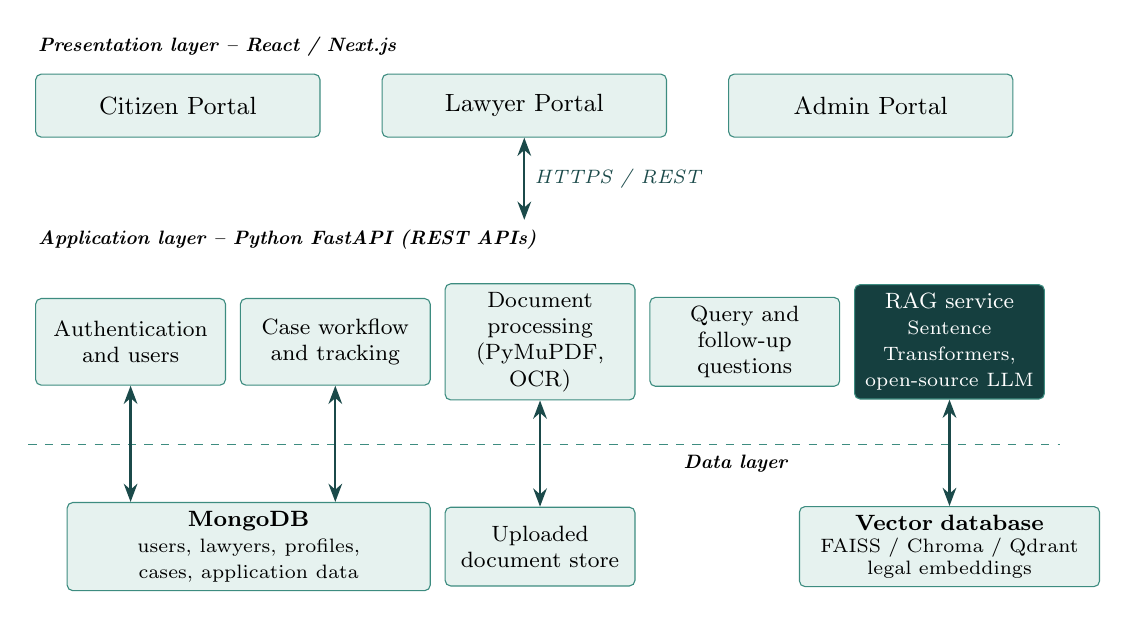
\begin{tikzpicture}[
  b/.style={wstep,text width=2.2cm,minimum height=1.1cm},
  p/.style={wstep,text width=3.4cm,minimum height=0.8cm,font=\small},
  lab/.style={font=\scriptsize\bfseries\itshape,anchor=west}]
  % presentation
  \node[p] (cp) at (0,7.0) {Citizen Portal};
  \node[p] (lp) at (4.4,7.0) {Lawyer Portal};
  \node[p] (ap) at (8.8,7.0) {Admin Portal};
  \node[lab] at (-1.9,7.75) {Presentation layer -- React / Next.js};
  % application
  \node[lab] at (-1.9,5.3) {Application layer -- Python FastAPI (REST APIs)};
  \node[b] (auth) at (-0.6,4) {Authentication and users};
  \node[b] (case) at (2,4) {Case workflow and tracking};
  \node[b] (doc) at (4.6,4) {Document processing (PyMuPDF, OCR)};
  \node[b] (q) at (7.2,4) {Query and follow-up questions};
  \node[dark,text width=2.2cm,minimum height=1.1cm] (rag) at (9.8,4) {RAG service\\{\scriptsize Sentence Transformers, open-source LLM}};
  \draw[{Stealth}-{Stealth},thick,color=headteal] (lp.south) -- node[right,font=\scriptsize\itshape]{HTTPS / REST} (4.4,5.55);
  % data
  \draw[dashed,color=boxline] (-1.9,2.7) -- (11.2,2.7);
  \node[lab] at (6.3,2.45) {Data layer};
  \node[wstep,text width=4.4cm,minimum height=1.0cm] (mongo) at (0.9,1.4) {\textbf{MongoDB}\\{\scriptsize users, lawyers, profiles, cases, application data}};
  \node[wstep,text width=2.2cm,minimum height=1.0cm] (store) at (4.6,1.4) {Uploaded document store};
  \node[wstep,text width=3.6cm,minimum height=1.0cm,font=\scriptsize] (vdb) at (9.8,1.4) {{\footnotesize\textbf{Vector database}}\\FAISS / Chroma / Qdrant\\legal embeddings};
  \foreach \x in {auth,case} \draw[{Stealth}-{Stealth},thick,color=headteal] (\x.south) -- (\x.south |- mongo.north);
  \draw[{Stealth}-{Stealth},thick,color=headteal] (doc.south) -- (store.north);
  \draw[{Stealth}-{Stealth},thick,color=headteal] (rag.south) -- (vdb.north);
\end{tikzpicture}
\caption{System architecture}
\label{fig:arch}
\end{figure}

\subsection*{RAG Pipeline}
RAG stands for Retrieval-Augmented Generation. A simple way to think about it is an open-book exam: before the model writes anything, it has to open the verified law book, find the right pages, and answer from those pages only. Figure~\ref{fig:rag} shows the two phases.
\begin{itemize}
  \item \textbf{Offline phase (building the knowledge base).} This happens once, before any user arrives. We collect verified Pakistani legal sources, clean and check them, and extract the text with PyMuPDF or OCR. The text is then cut into section-wise chunks, each tagged with metadata such as the act and section number. Sentence Transformers turns every chunk into an embedding, and the result is stored in the vector database.
  \item \textbf{Online phase (answering a case).} This happens every time someone asks for help. The system takes the case description and answers, and asks follow-up questions if facts are missing. It then turns the question into an embedding and finds the closest legal sections in the vector database. Those sections, together with strict instructions to answer only from them, are sent to the open-source LLM. The draft answer is checked against its sources and citations, and the user receives a plain-language answer with the citations attached.
\end{itemize}

\begin{figure}[H]
\centering
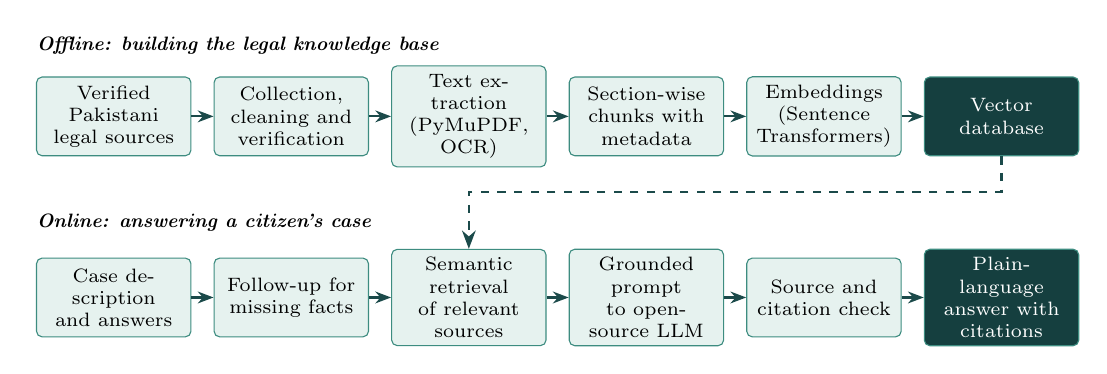
\begin{tikzpicture}[node distance=0.28cm, s/.style={wstep,text width=1.75cm,minimum height=1.0cm,font=\scriptsize}, d/.style={dark,text width=1.75cm,minimum height=1.0cm,font=\scriptsize}]
  \node[font=\scriptsize\bfseries\itshape,anchor=west] at (-1.1,0.9) {Offline: building the legal knowledge base};
  \node[s] (o1) at (0,0) {Verified Pakistani legal sources};
  \node[s,right=of o1] (o2) {Collection, cleaning and verification};
  \node[s,right=of o2] (o3) {Text extraction (PyMuPDF, OCR)};
  \node[s,right=of o3] (o4) {Section-wise chunks with metadata};
  \node[s,right=of o4] (o5) {Embeddings (Sentence Transformers)};
  \node[d,right=of o5] (o6) {Vector database};
  \foreach \a/\b in {o1/o2,o2/o3,o3/o4,o4/o5,o5/o6} \draw[flow] (\a) -- (\b);
  \node[font=\scriptsize\bfseries\itshape,anchor=west] at (-1.1,-1.35) {Online: answering a citizen's case};
  \node[s] (n1) at (0,-2.3) {Case description and answers};
  \node[s,right=of n1] (n2) {Follow-up for missing facts};
  \node[s,right=of n2] (n3) {Semantic retrieval of relevant sources};
  \node[s,right=of n3] (n4) {Grounded prompt to open-source LLM};
  \node[s,right=of n4] (n5) {Source and citation check};
  \node[d,right=of n5] (n6) {Plain-language answer with citations};
  \foreach \a/\b in {n1/n2,n2/n3,n3/n4,n4/n5,n5/n6} \draw[flow] (\a) -- (\b);
  \draw[-{Stealth},dashed,color=headteal,thick] (o6.south) -- ++(0,-0.45) -| (n3.north);
\end{tikzpicture}
\caption{RAG pipeline --- offline knowledge base preparation and online answering}
\label{fig:rag}
\end{figure}

\begin{example}[Example: what retrieval looks like for Ali]
Ali's question, ``My landlord says I must leave in 7 days,'' is turned into an embedding and compared with every section in the knowledge base. The closest matches are the rent law sections on eviction and notice, along with the rules on tenancy agreements, so those are passed to the LLM. A section on child custody would score very low and is never sent. The LLM never searches the database itself; it only sees what the RAG service hands to it.
\end{example}

\subsection*{Development Environment, Operating Systems and Network Protocol}
\begin{itemize}
  \item \textbf{Development environment.} We will use ordinary code editors and Git for version control, Python virtual environments for the backend, and Node.js for the frontend.
  \item \textbf{Operating systems.} Since Python, Node.js and MongoDB all run on Windows, Linux and macOS, each of us can work on whatever machine we have. For deployment we plan to use a Linux server.
  \item \textbf{Network protocol.} The frontend and backend talk through REST APIs over HTTP/HTTPS, with HTTPS keeping data safe while it travels.
\end{itemize}

\section{Project Work Breakdown}
We have broken the project into 20 work packages (Table~\ref{tab:wbs}). Keeping them small and clearly described makes it easier to track progress and know who is responsible for what.

\begin{longtable}{|>{\centering\arraybackslash}p{0.8cm}|L{4.6cm}|L{8.6cm}|}
\caption{Work breakdown structure}\label{tab:wbs}\\
\hline
\headrow \thd{No.} & \thd{Work package} & \thd{Description} \\ \hline
\endfirsthead
\hline
\headrow \thd{No.} & \thd{Work package} & \thd{Description} \\ \hline
\endhead
1 & Project planning & Define scope, roles, schedule and tools. \\ \hline
\rowcolor{rowtint}2 & Requirements analysis & Collect user, lawyer and admin requirements and prepare the feature list. \\ \hline
3 & Legal research & Study the property and family dispute areas to understand the legal issues involved. \\ \hline
\rowcolor{rowtint}4 & Legal source identification & Select the verified Pakistani legal sources to be used. \\ \hline
5 & Legal corpus collection & Collect the selected sources into one corpus. \\ \hline
\rowcolor{rowtint}6 & Data cleaning and verification & Clean the text and check the reliability of each source. \\ \hline
7 & Document processing & Extract PDF text with PyMuPDF and prepare OCR for scanned files. \\ \hline
\rowcolor{rowtint}8 & Vector database / embedding preparation & Split text into chunks, create embeddings and store them in the vector database. \\ \hline
9 & RAG baseline & Build the first working retrieval and grounded generation pipeline with citations. \\ \hline
\rowcolor{rowtint}10 & Backend development & Develop FastAPI services, authentication and MongoDB integration. \\ \hline
11 & Frontend development & Develop the citizen, lawyer and admin portals. \\ \hline
\rowcolor{rowtint}12 & Case workflow & Implement case creation, follow-up questions and status tracking. \\ \hline
13 & Lawyer directory & Implement lawyer profiles, verification, search and filters. \\ \hline
\rowcolor{rowtint}14 & Document / OCR integration & Integrate upload, text extraction and the evidence checklist into the application. \\ \hline
15 & System integration & Connect the frontend, backend, databases and RAG service. \\ \hline
\rowcolor{rowtint}16 & Testing & Perform functional and system testing and report bugs. \\ \hline
17 & Security testing & Check access control, authentication and data protection. \\ \hline
\rowcolor{rowtint}18 & Evaluation & Compare the standard LLM with the RAG system and measure usability with SUS. \\ \hline
19 & Deployment & Set up the final system on a server. \\ \hline
\rowcolor{rowtint}20 & Documentation and defense preparation & Prepare reports, presentation and defense. \\ \hline
\end{longtable}

\subsection*{Team Assignment}
We work as one team, but each of us owns one main area (Table~\ref{tab:team}).

\begin{table}[H]
\centering
\caption{Team assignment}
\label{tab:team}
\begin{tabular}{|L{3.4cm}|L{5.6cm}|L{5.0cm}|}
\hline
\headrow \thd{Member} & \thd{Primary responsibility} & \thd{Collaborative work} \\ \hline
\textbf{Muhammad Nabeel} & Development: full-stack, backend/frontend integration, RAG and system integration & Research, data, integration, testing, documentation \\ \hline
\rowcolor{rowtint}\textbf{Ashir Qureshi} & Development: full-stack, frontend/backend development, feature implementation and integration & Research, data, integration, testing, documentation \\ \hline
\textbf{Muhammad Sharjeel} & QA/Testing: test planning, functional and system testing, bug identification, quality assurance & Research, data, testing, documentation, integration support \\ \hline
\end{tabular}
\end{table}

That said, a lot of the work is shared. All three of us take part in research, gathering requirements, studying the legal domain, finding and collecting legal sources, cleaning and verifying data, looking at competitors, planning features, discussing the system and UI/UX design, documentation, integration, testing, solving problems as they come up, and preparing for the final presentation and defense.

\section{Project Timeline}
We have planned the work over seven months (M1 to M7):
\begin{itemize}
  \item \textbf{M1--M2:} legal research, source identification, corpus collection, and cleaning and verification.
  \item \textbf{M3:} document processing, embeddings and the RAG baseline.
  \item \textbf{M4--M5:} backend, frontend, case workflow, lawyer directory and system integration.
  \item \textbf{M6:} security testing and evaluation.
  \item \textbf{M7:} deployment and defense.
\end{itemize}
Exact dates are not fixed yet. Planning, requirements and documentation will run alongside the technical work throughout, and we will start testing as soon as the first features are connected.

\newcommand{\g}{\cellcolor{gantt}}
\begin{table}[H]
\centering
\caption{Seven-month project timeline (shaded cells show active work)}
\label{tab:timeline}
\renewcommand{\arraystretch}{1.25}
\begin{tabular}{|>{\centering\arraybackslash}p{0.7cm}|L{5.6cm}|*{7}{>{\centering\arraybackslash}p{0.75cm}|}}
\hline
\headrow \thd{No.} & \thd{Task} & \thd{M1} & \thd{M2} & \thd{M3} & \thd{M4} & \thd{M5} & \thd{M6} & \thd{M7} \\ \hline
1 & Project planning & \g & & & & & & \\ \hline
2 & Requirements analysis & \g & & & & & & \\ \hline
3 & Legal research & \g & \g & & & & & \\ \hline
4 & Legal source identification & \g & \g & & & & & \\ \hline
5 & Legal corpus collection & \g & \g & & & & & \\ \hline
6 & Data cleaning and verification & \g & \g & & & & & \\ \hline
7 & Document processing & & \g & \g & & & & \\ \hline
8 & Vector database / embedding preparation & & \g & \g & & & & \\ \hline
9 & RAG baseline & & & \g & & & & \\ \hline
10 & Backend development & & & & \g & \g & & \\ \hline
11 & Frontend development & & & & \g & \g & & \\ \hline
12 & Case workflow & & & & \g & \g & & \\ \hline
13 & Lawyer directory & & & & \g & \g & & \\ \hline
14 & Document / OCR integration & & & & \g & \g & & \\ \hline
15 & System integration & & & & \g & \g & & \\ \hline
16 & Testing & & & & \g & \g & \g & \\ \hline
17 & Security testing & & & & & & \g & \\ \hline
18 & Evaluation & & & & & & \g & \\ \hline
19 & Deployment & & & & & & & \g \\ \hline
20 & Documentation and defense preparation & \g & \g & \g & \g & \g & \g & \g \\ \hline
\end{tabular}
\end{table}

\end{document}
